\documentclass[sensors,article,submit,moreauthors,pdftex]{Definitions/mdpi}

\firstpage{1}
\makeatletter
\setcounter{page}{\@firstpage}
\makeatother
\pubvolume{xx}
\issuenum{1}
\articlenumber{5}
\pubyear{2026}
\copyrightyear{2026}
\history{Received: date; Accepted: date; Published: date}

\graphicspath{{figures/}}
\DeclareGraphicsExtensions{.pdf,.png,.eps}

\usepackage{amsmath}
\usepackage{booktabs}
\usepackage{subcaption}
\usepackage{multirow}
\usepackage{siunitx}
\setlength{\emergencystretch}{2em}

\Title{AERIS: Environment-Aware Hierarchical Routing for Reliable Wireless Sensor Networks under Realistic Channel Conditions}

\Author{Kangrui Li $^{1,}$*, Xiaobo Zhang $^{1}$ and Junyi Lin $^{1}$}
\AuthorNames{Kangrui Li, Xiaobo Zhang and Junyi Lin}
\address{$^{1}$ \quad Faculty of Automation, Guangdong University of Technology, Guangzhou 510006, China}
\corres{Correspondence: 1403073295@mails.gdut.edu.cn}

\abstract{This paper evaluates AERIS, a lightweight hierarchical routing protocol for wireless sensor networks under heterogeneous channel conditions. The primary metric is \texttt{pdr\_expected} (base-station delivered packets divided by expected source packets). In the publication-tier 100-node regime (four environments, 30 seeds per environment), AERIS achieves the highest mean packet delivery ratio within the tested baseline set (LEACH, PEGASIS, HEED, and TEEN). In the current large-scale frozen matrix (100--1000 nodes, four environments, 1000 replicates per environment-node-protocol cell), AERIS remains the highest-mean protocol in all 24 environment-scale cells. Ablation results still indicate environment-dependent module effects: Gateway is positive in harsh environments and near-neutral in indoor office, whereas CAS does not provide a uniformly positive marginal effect. Hop-based latency analysis shows AERIS near two hops, while PEGASIS remains above 31 hops due to chain traversal. NS-3 evidence is used strictly as trend-level cross-platform validation (AERIS vs LEACH), not as a numerical-equivalence proof. All conclusions are explicitly bounded to the tested protocol set, environment taxonomy, metric definition, and sample-size regime, and a simulator-rigor refinement path is tracked as ongoing work.}

\keyword{wireless sensor networks; reliable routing; hierarchical protocol; packet delivery ratio; scalability; reproducible evaluation}

\begin{document}

\section{Introduction}
Wireless sensor network (WSN) routing is classically optimized for energy reduction, but practical deployments also require stable delivery under heterogeneous channels \cite{Akyildiz2002Survey,Rault2016Energy,Kandris2020}. This creates a multi-objective tension among reliability, hop-based latency, and energy use. Existing protocols represent distinct operating points: LEACH emphasizes clustered forwarding \cite{Heinzelman2000LEACH}, PEGASIS emphasizes chain-based aggregation \cite{Lindsey2002PEGASIS}, HEED emphasizes residual-energy-aware head selection \cite{Younis2004HEED}, and TEEN emphasizes event-triggered reporting \cite{Manjeshwar2001TEEN}. Prior channel studies also show that low-power links can be asymmetric and environment-sensitive under realistic propagation conditions \cite{Zuniga2004,Zuniga2007Asymmetry,Baccour2012RLQE}.

AERIS is designed as a lightweight hierarchical protocol that prioritizes reliability under realistic channel variability. The design objective is not universal dominance; rather, it is robust performance across multiple channel environments while preserving deployability on resource-constrained nodes.

\subsection*{Contributions and Scope Boundaries}
This manuscript makes three scoped contributions. First, it provides publication-tier evidence for multi-environment reliability comparison at 100 nodes and environment-stratified scalability analysis up to 1000 nodes. Second, it quantifies module-level behavior with ablation under the same channel taxonomy. Third, it adds cross-platform trend validation in NS-3 for AERIS versus LEACH. The manuscript explicitly does not claim universal protocol superiority, five-protocol cross-platform ranking, or cross-platform numerical equivalence. Every inference is constrained to the reported metric, environment set, baseline set, and sample-size regime, and no claim is extrapolated beyond the audited matrices.

\section{Related Work}
Classical WSN protocols (LEACH, PEGASIS, HEED, TEEN) provide foundational routing mechanisms but show different failure modes under harsh channels and larger scales \cite{Heinzelman2002LEACH,Lindsey2002PEGASIS,Younis2004HEED,Kandris2020}. Chain-based aggregation can reduce per-hop transmission effort but increases end-to-end hop count. Cluster-based approaches can reduce hop count but may become sensitive to uplink quality and head placement.

Recent adaptive or learning-based methods improve specific settings but often require heavier runtime or training overhead \cite{Ren2024,Okine2024,Chen2023Survey}. Recent Sensors/IoT studies also report robust gains from context-aware or hybrid routing under constrained networks \cite{ElFouly2023ILP,Dan2024EMRAR,Bhukya2025Hybrid}. These results motivate explicit environmental adaptation in protocol design while keeping inference and control logic lightweight. In this manuscript, the focus is a rule-based protocol with explicit reproducibility constraints and auditable experiment metadata.

\section{System Model and Protocol}
\subsection{Metric Definition}
The primary metric is
\begin{equation}
\mathrm{PDR}_{\mathrm{expected}} = \frac{\mathrm{bs\_delivered}}{\mathrm{source\_packets\_expected}}.
\end{equation}
All publication conclusions in this draft are based on this metric.

\subsection{AERIS Architecture}
AERIS combines three components:
\begin{enumerate}
\item Context-Adaptive Switching (CAS) for mode control,
\item Skeleton backbone for hierarchical forwarding,
\item Gateway coordination for CH-to-BS reinforcement.
\end{enumerate}
Gateway candidate scoring follows a weighted rule
\begin{equation}
\mathrm{Score}_i = \alpha E_i + \beta C_i + \gamma L_i
\end{equation}
where $E_i$ is residual energy, $C_i$ is centrality, and $L_i$ is link quality.

\section{Experimental Setup}
\subsection{Publication-Tier Settings}
\begin{itemize}
\item Simulator: Python implementation with logged provenance.
\item Channel environments: indoor\_office, indoor\_factory, outdoor\_urban, outdoor\_suburban.
\item Default node count: 100.
\item Seeds for multi-environment and ablation: 30 independent seeds.
\item Seeds for scalability: balanced frozen regime with n=1000 per environment-node-protocol cell (100--1000 nodes, 4 environments).
\item Baselines: LEACH, PEGASIS, HEED, TEEN.
\end{itemize}

\subsection{Evidence Scope}
The analysis is grounded in publication-tier multi-environment comparison, ablation, scalability, hop-based latency, energy-lifetime statistics, and NS-3 trend validation. Claims are constrained to this evidence scope. Cross-platform numerical equivalence is intentionally not claimed, and cross-regime numerical pooling is avoided.

\subsection{Statistical Methods}
For pairwise protocol comparisons, we use Welch's two-sample $t$-test because variance equality is not assumed across protocols and environments. Family-wise error control is handled by Holm correction within each reported comparison family. Effect size is reported with Hedges' $g$ and interpreted as small (0.2), medium (0.5), and large (0.8) in absolute value. Confidence intervals are reported as two-sided 95\% intervals. All significance statements in this manuscript are based on Holm-corrected $p$ values. For large-$n$ cells, interpretation is based jointly on corrected $p$ values, effect size, and absolute PDR delta.

\subsection{Reproducibility Controls}
All publication-tier scripts in this study use deterministic seed lists. They also enforce \texttt{force\_ctp\_reliable=False}. This guarantees that PDR reflects simulated delivery behavior rather than any reliability override. We report \texttt{pdr\_expected} as the primary metric and treat hop count as a latency proxy, not a wall-clock latency measurement. Significance statements are accepted only when consistent with the declared regime-specific sample size.

\section{Results}
\subsection{Multi-Environment Comparison at 100 Nodes (n=30)}
\begin{table}[H]
\caption{PDR by environment at 100 nodes (mean $\pm$ std; std follows the result-file convention with ddof=0).}
\label{tab:pdr100}
\centering
\resizebox{\linewidth}{!}{
\begin{tabular}{lccccc}
\toprule
Environment & AERIS & LEACH & PEGASIS & HEED & TEEN \\
\midrule
indoor\_office   & 0.9739$\pm$0.0047 & 0.5543$\pm$0.0401 & 0.9078$\pm$0.0166 & 0.9371$\pm$0.0076 & 0.8222$\pm$0.0044 \\
indoor\_factory  & 0.6031$\pm$0.0258 & 0.1614$\pm$0.0209 & 0.1928$\pm$0.0255 & 0.2326$\pm$0.0263 & 0.3113$\pm$0.0245 \\
outdoor\_urban   & 0.3745$\pm$0.0354 & 0.0552$\pm$0.0127 & 0.0542$\pm$0.0117 & 0.0635$\pm$0.0121 & 0.1201$\pm$0.0183 \\
outdoor\_suburban& 0.7451$\pm$0.0193 & 0.2703$\pm$0.0272 & 0.3382$\pm$0.0329 & 0.4221$\pm$0.0313 & 0.4752$\pm$0.0236 \\
\bottomrule
\end{tabular}
}
\end{table}

At 100 nodes, AERIS ranks first in all four tested environments within the evaluated baseline set (LEACH, PEGASIS, HEED, and TEEN). This claim is restricted to the 100-node matrix and should not be generalized to the 1000-node regime.

\begin{figure}[H]
\centering
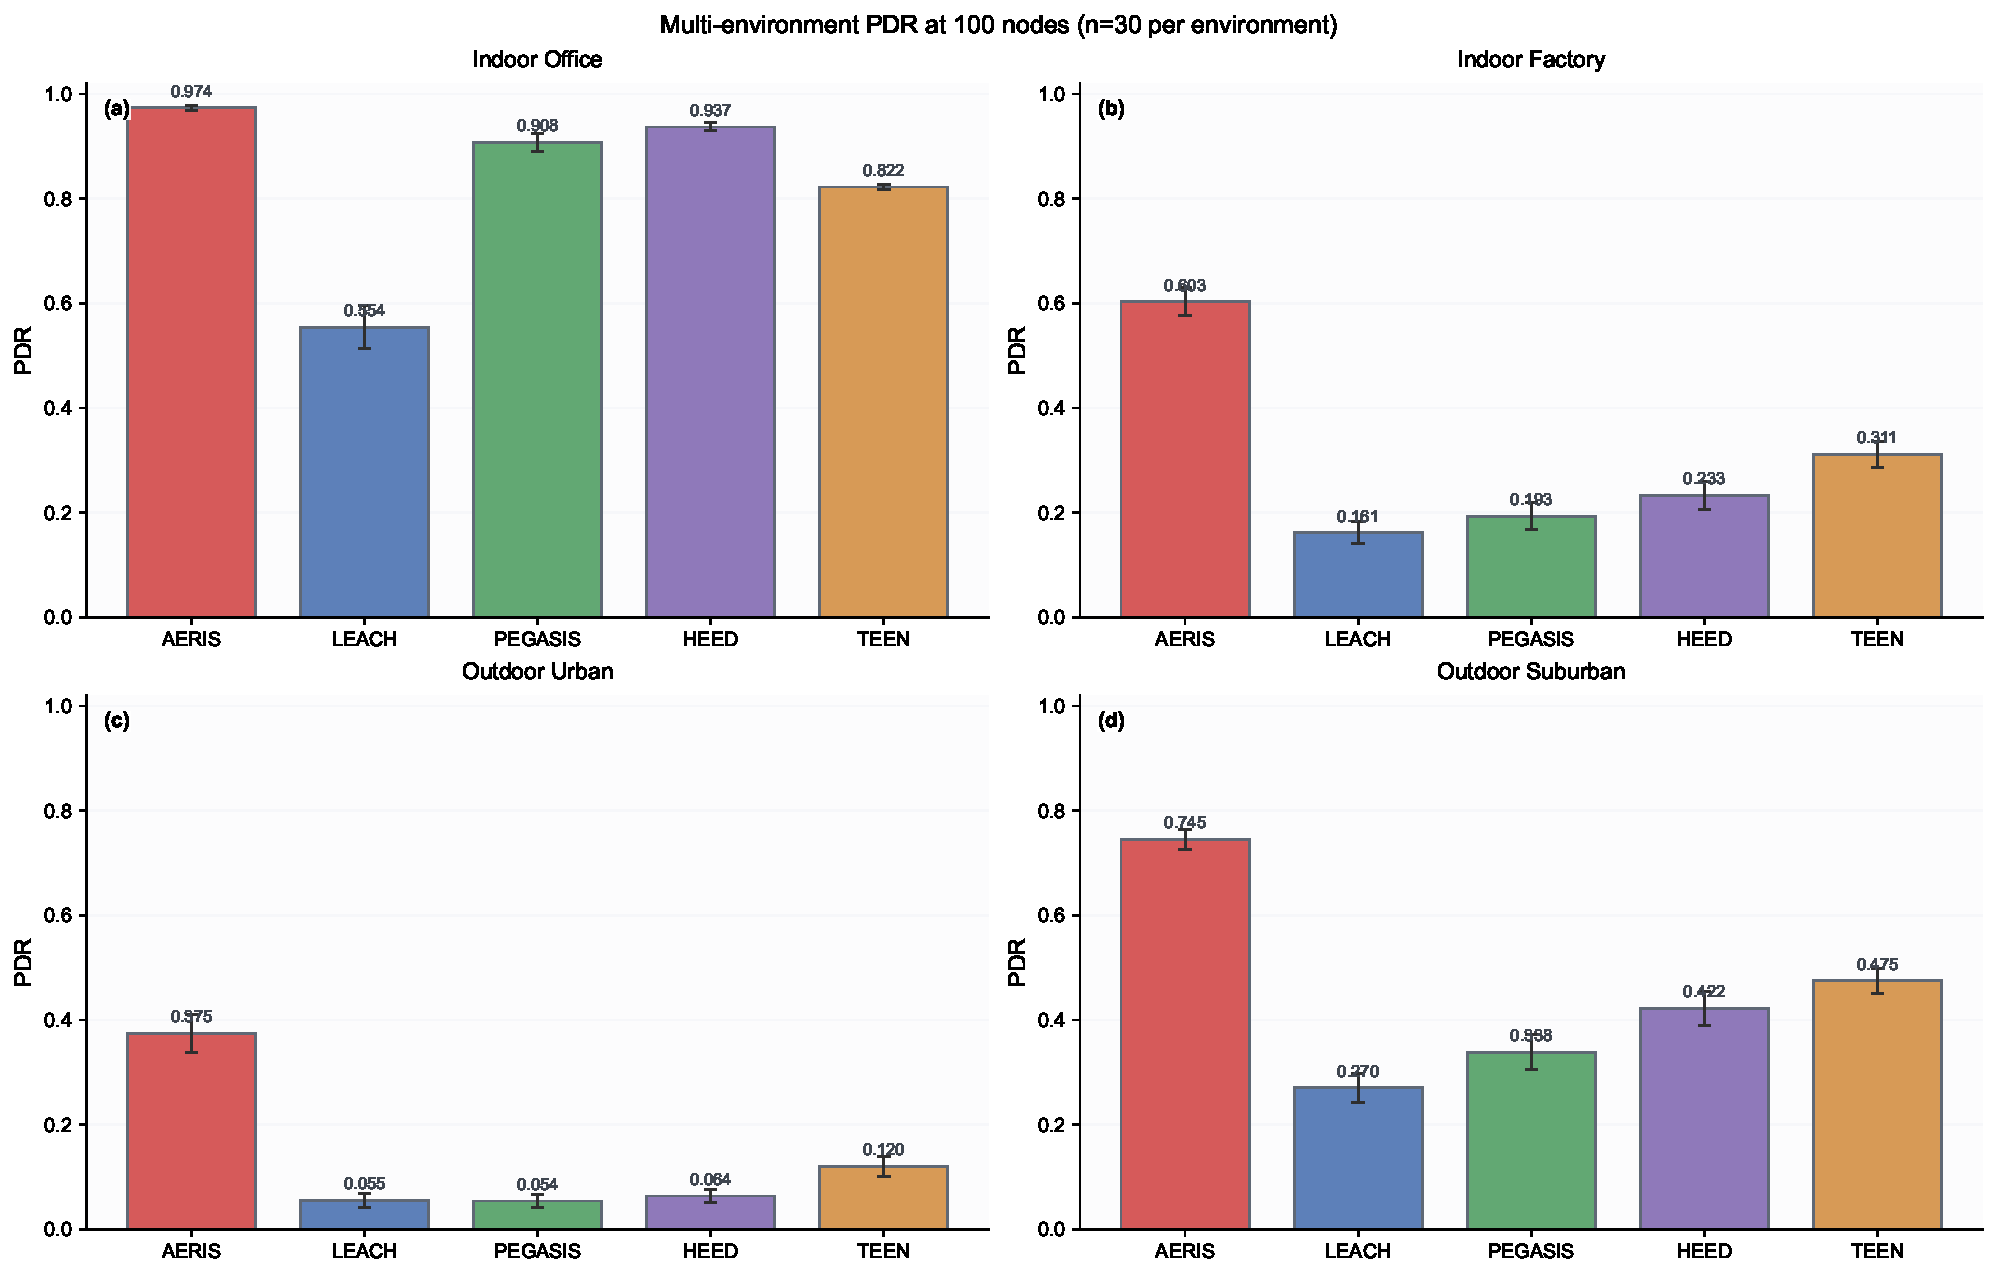
\includegraphics[width=0.95\textwidth]{fig1_env_pdr_panel_20260215_s23.pdf}
\caption{PDR comparison panel at 100 nodes (4 environments, n=30).}
\label{fig:env_panel}
\end{figure}

\subsection{Ablation: Environment-Dependent Effects (n=30)}
\begin{table}[H]
\caption{Full vs no\_gateway PDR (mean $\pm$ std; std reported as population standard deviation, ddof=0).}
\label{tab:ablation_gateway}
\centering
\begin{tabular}{lccc}
\toprule
Environment & Full & no\_gateway & Delta (no\_gateway - full) \\
\midrule
indoor\_office    & 0.9739$\pm$0.0047 & 0.9741$\pm$0.0036 & +0.0002 \\
indoor\_factory   & 0.6031$\pm$0.0258 & 0.5806$\pm$0.0215 & -0.0225 \\
outdoor\_urban    & 0.3745$\pm$0.0354 & 0.3534$\pm$0.0301 & -0.0212 \\
outdoor\_suburban & 0.7451$\pm$0.0193 & 0.7306$\pm$0.0264 & -0.0146 \\
\bottomrule
\end{tabular}
\end{table}

Gateway is positive in three environments and near-neutral in indoor\_office. CAS is not consistently positive across environments.
In indoor\_office, the Full-vs-no\_gateway gap is +0.0002 (absolute PDR), so this cell is treated as practically neutral.

\begin{figure}[H]
\centering
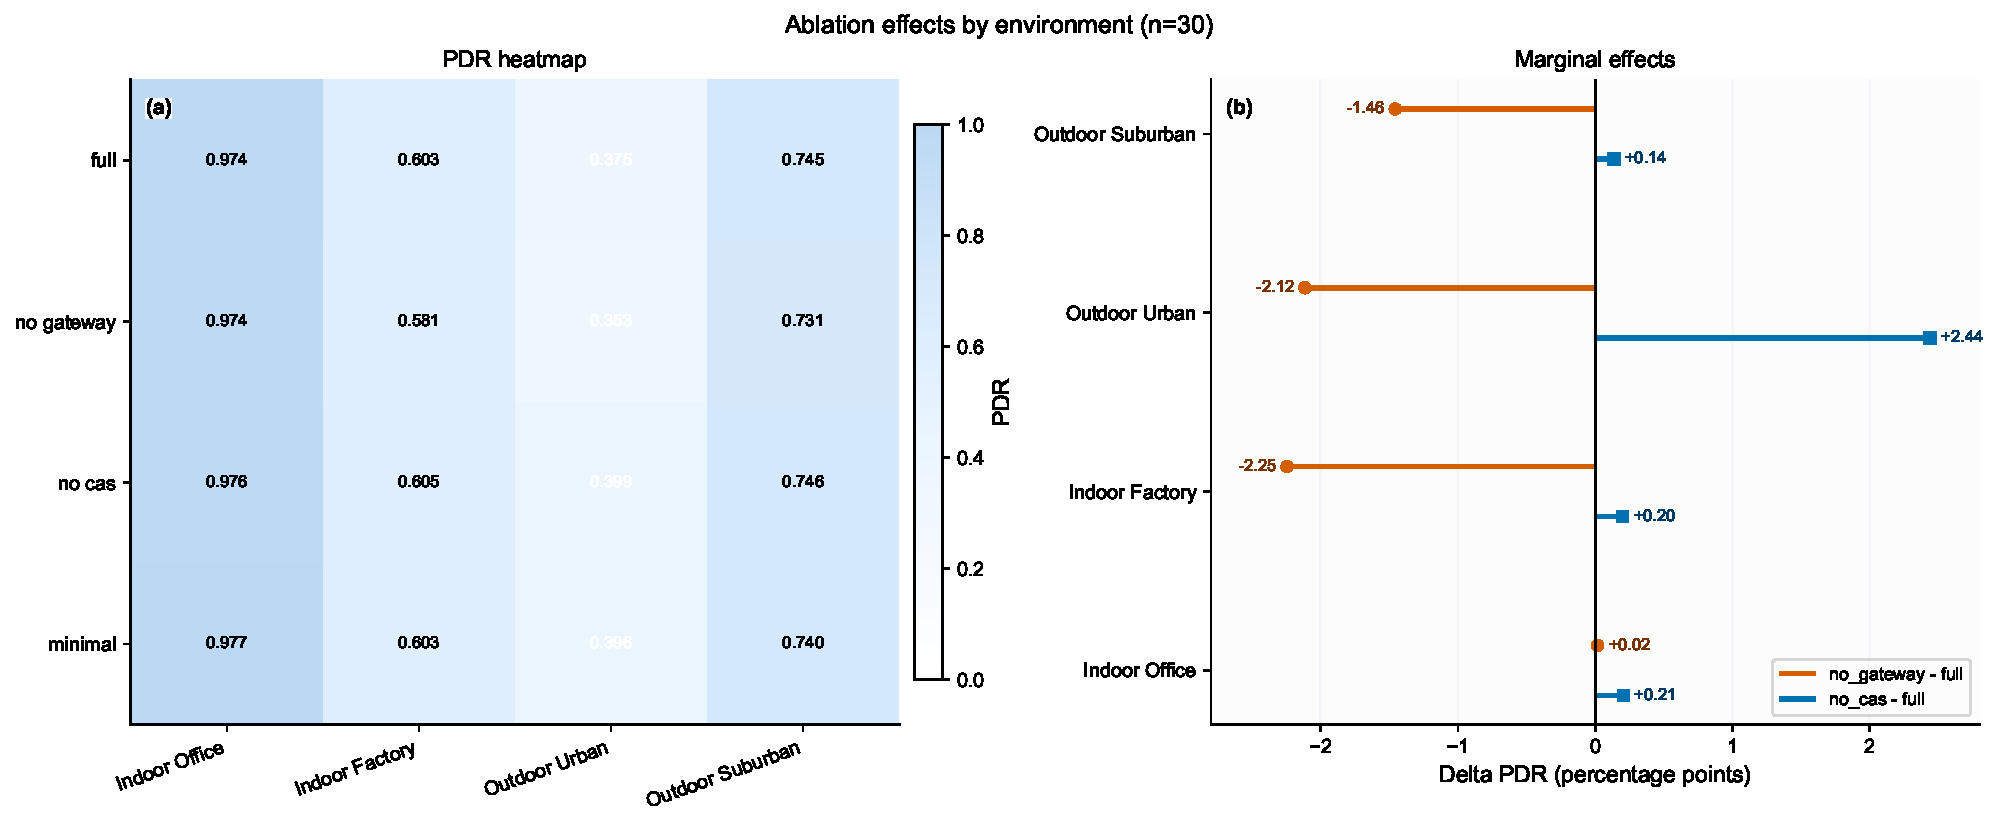
\includegraphics[width=0.95\textwidth]{fig2_ablation_panel_20260215_s23.pdf}
\caption{Ablation panel: heatmap and marginal effects (n=30).}
\label{fig:ablation_panel}
\end{figure}

\subsection{Scalability (100--1000 Nodes; Balanced n=1000 per Cell)}
\begin{table}[H]
\caption{PDR ranking at 1000 nodes from the balanced S8 frozen matrix (n=1000 per cell).}
\label{tab:scale1000}
\centering
\begin{tabular}{lcccccc}
\toprule
Environment & AERIS & LEACH & PEGASIS & HEED & TEEN & AERIS rank \\
\midrule
indoor\_office    & 0.9899 & 0.6282 & 0.8942 & 0.8915 & 0.8032 & 1st \\
indoor\_factory   & 0.9726 & 0.1884 & 0.1672 & 0.1634 & 0.2199 & 1st \\
outdoor\_urban    & 0.8846 & 0.0622 & 0.0497 & 0.0341 & 0.0662 & 1st \\
outdoor\_suburban & 0.9896 & 0.3048 & 0.2875 & 0.3232 & 0.3669 & 1st \\
\bottomrule
\end{tabular}
\end{table}

AERIS is first in all four environments in the current balanced S8 matrix. This statement remains regime-specific: it is bounded to the tested environment taxonomy, protocol set, and simulator assumptions.

\subsection{Statistical Robustness Snapshot (AERIS vs LEACH)}
\begin{table}[H]
\caption{Holm-corrected significance snapshot at 1000 nodes (AERIS vs strongest baseline in each environment).}
\label{tab:robust_snapshot}
\centering
\begin{tabular}{lcccccc}
\toprule
Environment & Nodes & $\Delta$PDR & Hedges' $g$ & Holm $p$ & Significant \\
\midrule
indoor\_office    & 1000 & +0.095705 (vs PEGASIS) & +4.1500 & $<10^{-300}$ & yes \\
indoor\_factory   & 1000 & +0.752703 (vs TEEN) & +138.5282 & $<10^{-300}$ & yes \\
outdoor\_urban    & 1000 & +0.818370 (vs TEEN) & +180.0377 & $<10^{-300}$ & yes \\
outdoor\_suburban & 1000 & +0.622649 (vs TEEN) & +98.9577 & $<10^{-300}$ & yes \\
\bottomrule
\end{tabular}
\end{table}

This snapshot highlights strong gains in harsh environments and a moderate but significant gain in indoor\_office under the current balanced matrix.
For very large sample sizes, practical interpretation in this study still follows both effect size and absolute PDR gap rather than significance labels alone.
The very large absolute values of Hedges' $g$ in harsh environments reflect both large mean gaps and low within-group variance under large sample sizes; they should be interpreted as magnitude indicators within this experiment design, not as cross-study constants.

\begin{figure}[H]
\centering
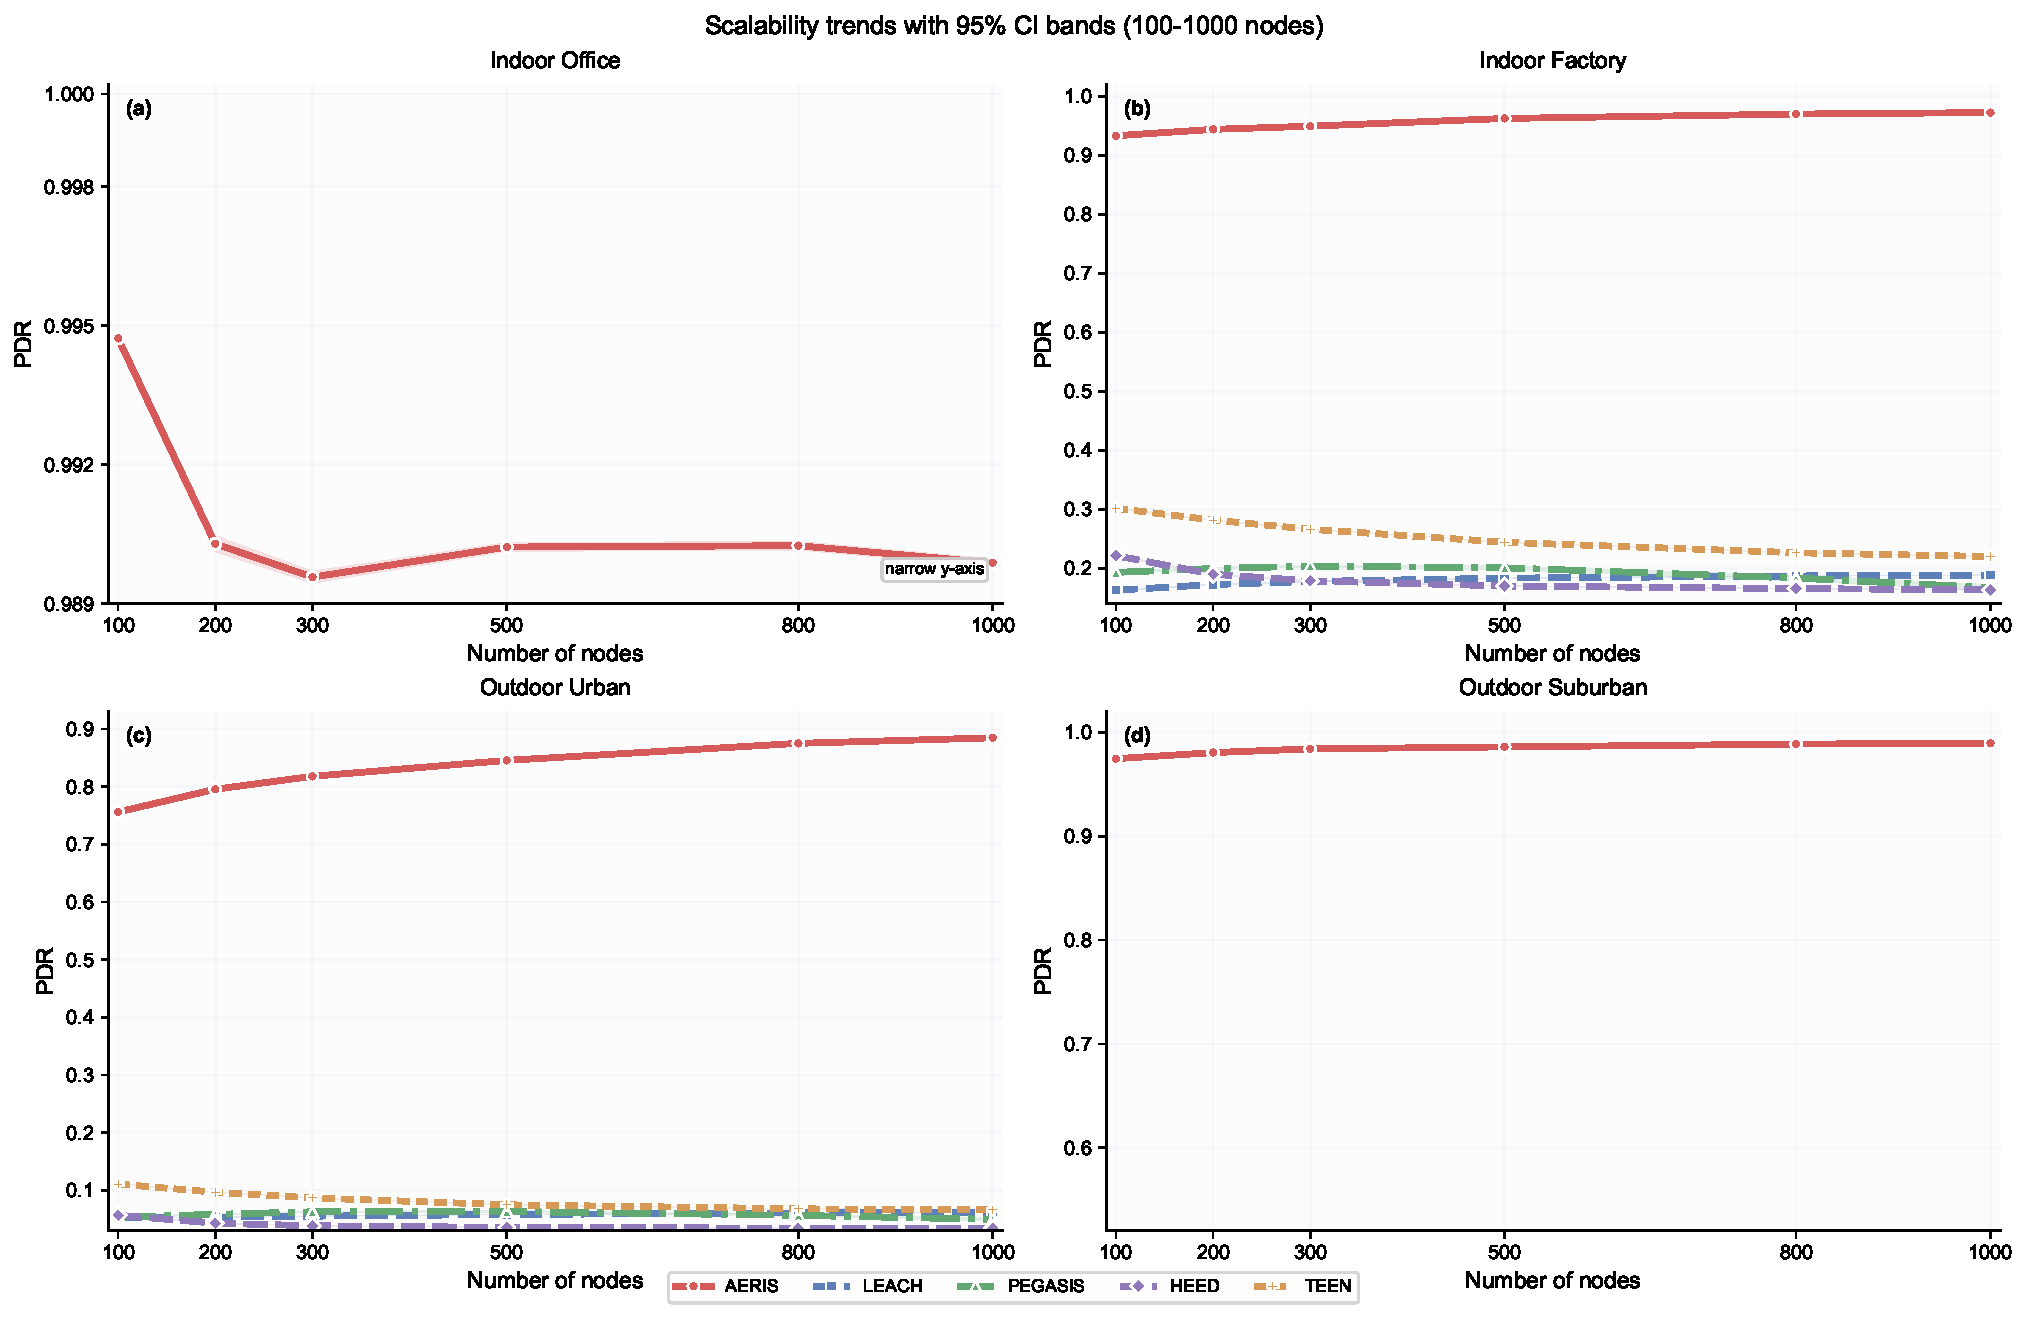
\includegraphics[width=0.95\textwidth]{fig3_scalability_panel_20260215_s23.pdf}
\caption{Scalability trends over node counts (balanced n=1000 per environment-node-protocol cell) with 95\% CI bands. The indoor\_office panel uses a narrowed y-axis window to expose non-zero ordering gaps near PDR=1.0.}
\label{fig:scalability_panel}
\end{figure}

\subsection{Hop-Based Latency and Trade-offs}
At 100 nodes (n=30), AERIS stays near two hops (1.97--1.99), while PEGASIS remains above 31 hops due to chain traversal. LEACH and TEEN show lower average hops because of protocol paths that allow direct-to-BS transmissions.

\begin{figure}[H]
\centering
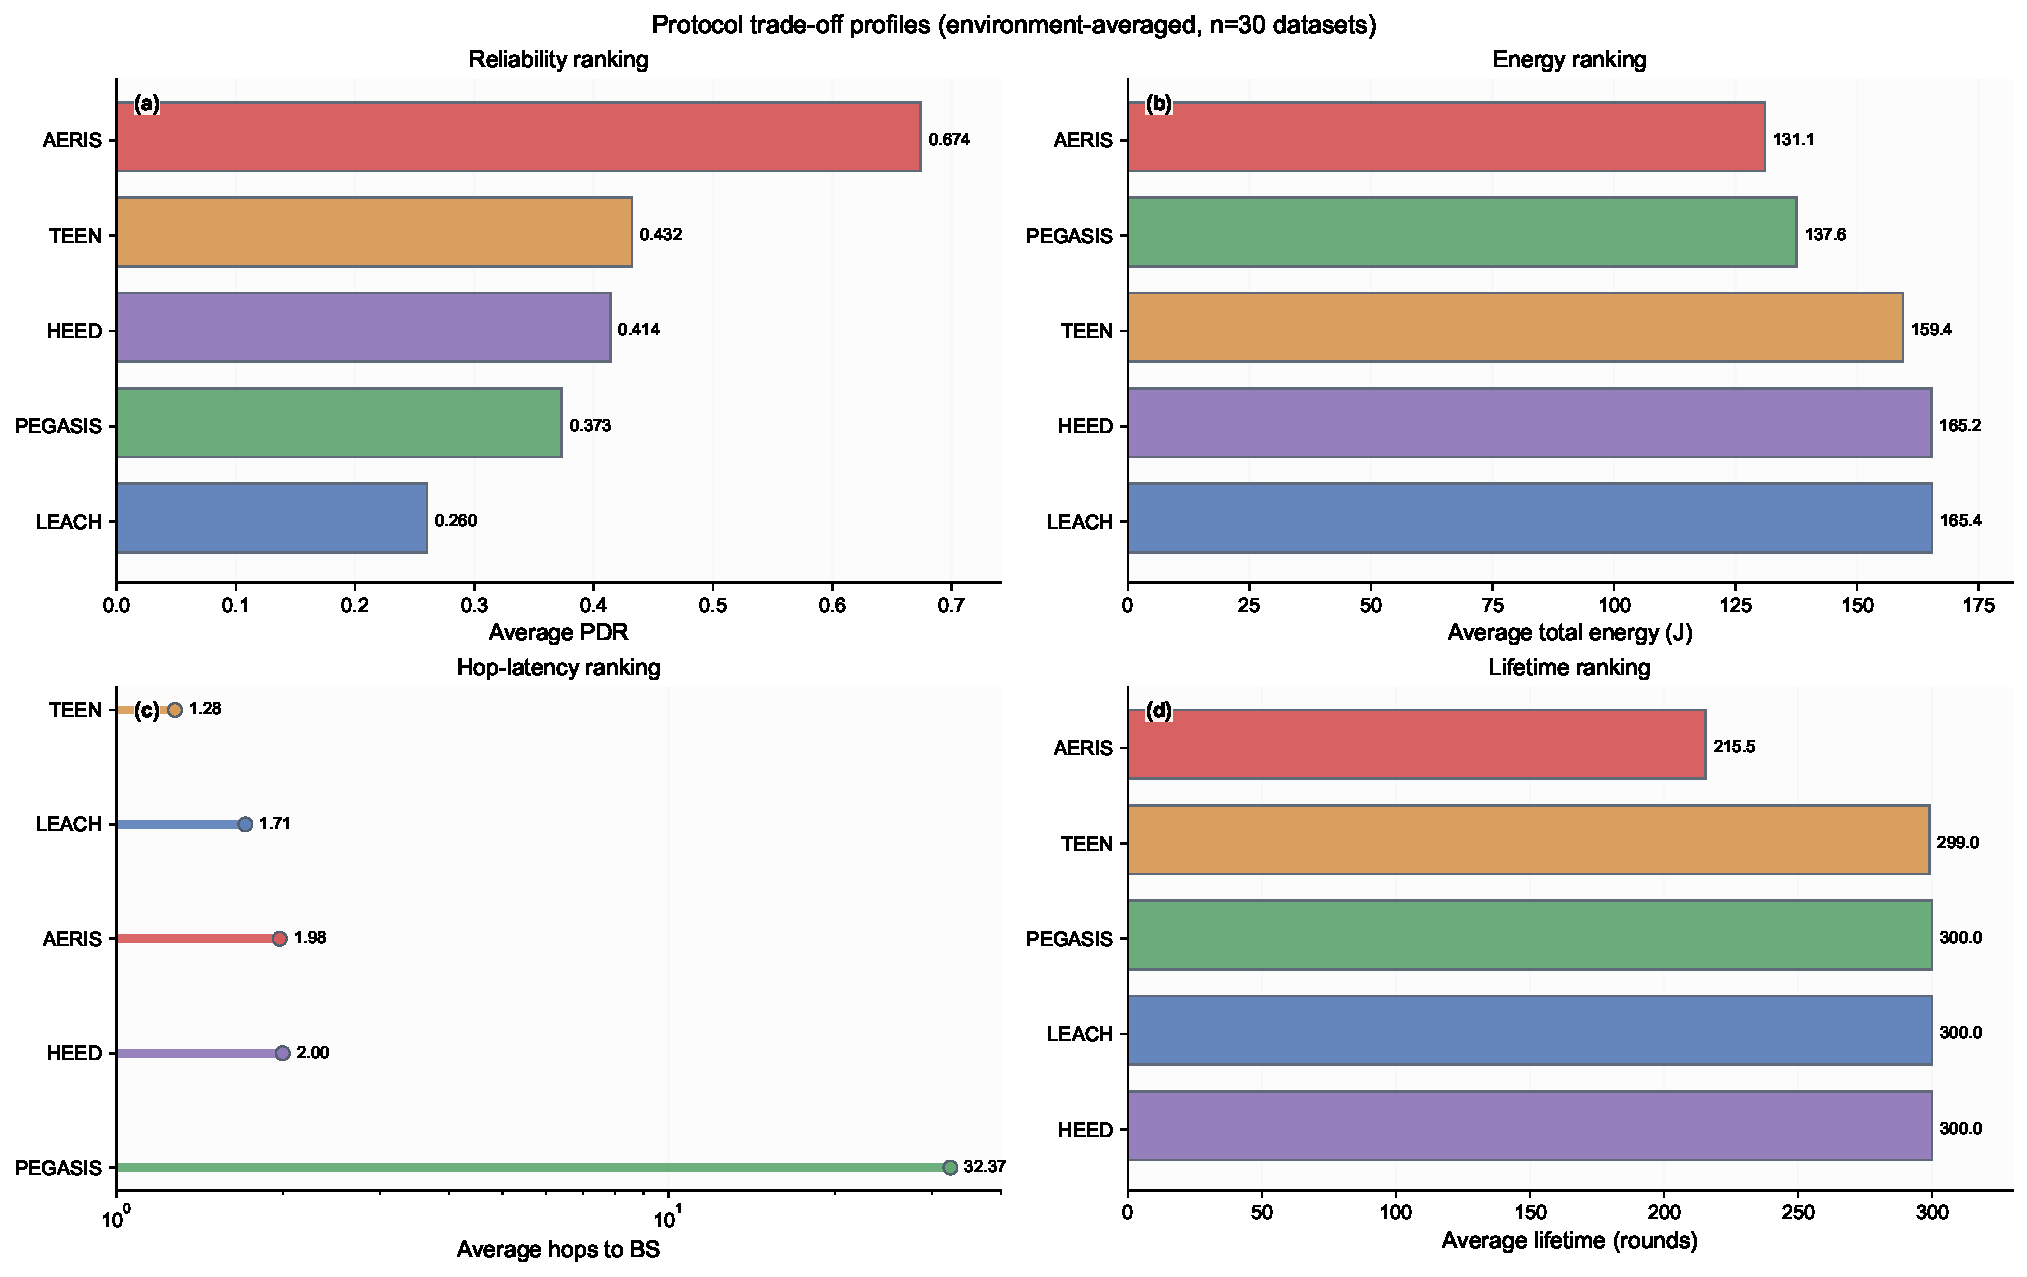
\includegraphics[width=0.95\textwidth]{fig4_tradeoff_panel_20260215_s23.pdf}
\caption{Trade-off panel from publication-tier data: reliability, energy, hop-based latency, and lifetime. The hop panel uses a logarithmic x-axis to keep low-hop and high-hop protocols visible in the same frame without overlap.}
\label{fig:tradeoff_panel}
\end{figure}

\subsection{NS-3 Trend Validation (AERIS vs LEACH, n=30)}
NS-3 validation is used as a cross-platform trend check rather than a numerical-equivalence proof. This block is restricted to AERIS-versus-LEACH and is not used for five-protocol cross-platform ranking. Under aligned multi-environment settings, AERIS is directionally not lower than LEACH in all tested environment-scale cells. At 100 nodes, significance is confirmed in 3/4 environments (indoor\_factory, outdoor\_urban, outdoor\_suburban), while indoor\_office remains non-significant. In the 300/500-node extension, all eight environment-scale comparisons are significant after Holm correction; with the 800/1000 extension included, non-significance remains confined to indoor\_office at 1000 nodes.

\begin{table}[H]
\caption{NS-3 trend-level validation at 100 nodes (AERIS vs LEACH, n=30; metric=\texttt{pdr\_expected}).}
\label{tab:ns3_trend}
\centering
\begin{tabular}{lccccc}
\toprule
Environment & AERIS & LEACH & Delta & Holm-corrected $p$ & Significance \\
\midrule
indoor\_office    & 0.9202 & 0.9185 & +0.0017 & 1.00 & no \\
indoor\_factory   & 0.6025 & 0.5336 & +0.0690 & $4.23\times10^{-25}$ & yes \\
outdoor\_urban    & 0.2064 & 0.1899 & +0.0165 & $3.41\times10^{-3}$ & yes \\
outdoor\_suburban & 0.7771 & 0.6921 & +0.0850 & $1.94\times10^{-30}$ & yes \\
\bottomrule
\end{tabular}
\end{table}

Scope note: this NS-3 block supports trend consistency only. The manuscript does not claim cross-platform numerical equivalence. Across 7 node counts and 4 environments, 25/28 AERIS-versus-LEACH comparisons are significant; the non-significant cells are indoor\_office at node counts 100, 200, and 1000.

\section{Discussion}
The evidence supports a scoped positioning rather than universal superiority. In the current reported matrices, AERIS is strong for reliability across heterogeneous channels, while all large-scale claims remain bounded to tested baselines, channel taxonomy, and simulator assumptions.

Practical interpretation requires separating statistical and engineering significance. At very large sample sizes, tiny absolute gaps can be statistically significant; therefore, conclusions in this paper rely on both corrected $p$ values and absolute PDR deltas. This is particularly relevant for indoor\_office at large scale, where ordering differences are small in magnitude.

Energy interpretation also requires caution: lower total energy can co-occur with shorter lifetime if a protocol terminates earlier. For this reason, reliability-energy statements are framed as conditioned trade-offs under fixed evaluation settings, not universal dominance claims.

The manuscript intentionally keeps three evidence blocks separate:
\begin{itemize}
\item 100-node multi-environment comparison,
\item large-scale regime (100--1000 nodes) with balanced n=1000 per cell,
\item NS-3 trend validation for AERIS versus LEACH only.
\end{itemize}
Cross-block numerical pooling is avoided. This separation is deliberate: the 100-node block and the 100--1000-node block answer different questions and therefore should not be merged into a single headline number.

\section{Limitations and Future Work}
\begin{itemize}
\item Current evidence is simulator-based.
\item NS-3 trend-level publication gate is completed; numerical equivalence is intentionally not claimed because of platform-depth differences.
\item NS-3 validation in this manuscript focuses on AERIS versus LEACH; full five-protocol cross-platform ranking remains future work.
\item The large-scale matrix is balanced at n=1000 per cell, but claims remain bounded to the tested channel taxonomy and simulator assumptions.
\item Reported gains are bounded to the tested baseline set and channel taxonomy.
\item Hop count is reported as a route-length proxy, not as a wall-clock latency benchmark under full MAC scheduling.
\item Additional topology families (corridor, hotspot) and hardware-in-the-loop validation remain pending.
\end{itemize}

\section{Conclusion}
AERIS provides a reliability-oriented routing option for heterogeneous WSN channels. In the publication-tier 100-node matrix, it achieves the highest mean PDR within the tested baseline set across all four environments. In the current balanced large-scale frozen matrix (100--1000 nodes, n=1000 per cell), AERIS remains the highest-mean protocol in all tested environments and scales. NS-3 confirms trend consistency for AERIS versus LEACH and is used strictly as trend-level evidence. Gateway effects are environment-dependent and CAS effects are mixed; therefore, the final claim is explicitly bounded to the tested protocol set, environment taxonomy, metric definition, and sample-size regimes.

\authorcontributions{Conceptualization, X.Z. and K.L.; methodology, K.L. and J.L.; software, K.L.; validation, X.Z. and J.L.; writing---original draft preparation, K.L.; writing---review and editing, X.Z.; supervision, X.Z.}
\funding{This research received no external funding.}
\conflictsofinterest{The authors declare no conflict of interest.}
\section*{Data Availability Statement}
The datasets, scripts, manuscript sources, figure-generation code, and provenance sidecar records (including commit identifiers and script hashes) supporting this study are available from the corresponding author and will be released in the public project repository upon final publication.

\reftitle{References}
\bibliography{bibliography}

\end{document}
